\documentclass[10pt]{article}





\usepackage[margin=1in]{geometry}
\usepackage{hyperref}
\usepackage{titling}
\usepackage{sectsty}
\sectionfont{\fontsize{11}{15}\selectfont}
\subsectionfont{\fontsize{11}{15}\selectfont}
\usepackage{titlesec}
\titlespacing*{\section}{0pt}{0.2\baselineskip}{0.2\baselineskip}
\usepackage{enumitem}

\usepackage{amsthm}
\usepackage{amssymb}
\usepackage{amsmath}
\usepackage{indentfirst} % Indent the first paragraph after sections
\usepackage{tcolorbox}
\tcbuselibrary{theorems,skins}
\usepackage{caption}
\DeclareCaptionFont{bold}{\bfseries}
\captionsetup[table]{labelfont={sf,bold}}
\usepackage{float}




\theoremstyle{definition}
\newtheorem{definition}{Definition}[section]
\newtcbtheorem[
  number within=section
]{problem}{Problem Formulation}{
  enhanced,
  frame hidden,
  colback=white,
  borderline west={2pt}{0pt}{gray!60},
  fonttitle=\bfseries,
  coltitle=black,
  before skip=5pt,   % reduce space before
  after skip=8pt,    % reduce space after
  top=2pt,           % reduce top padding
  bottom=2pt         % reduce bottom padding
}{pr}





\begin{document}
\setlength{\droptitle}{-7em}
\title{A Unified View of Frequency Estimation and their Attacks on Local Differential Privacy}



\author{Al Mehdi Saadat Chowdhury\thanks{CSE PhD 3rd year} \and Dhaval Pankaj Tanna\thanks{CSE Master's 2nd year}
\and Deepak Vellanki\thanks{CSE Master's 2nd year} \and Chirag Manjeshwar\thanks{CSE Master's 2nd year}}

% <-this % stops a space
%




\date{}
\maketitle
\vspace*{-1cm}





\begin{abstract}%
Generating meaningful statistical summaries without compromising individual privacy is a central challenge in data analysis. Local Differential Privacy (LDP) addresses this by allowing users to perturb their data before aggregation, but existing frequency estimation protocols are diverse and lack a common framework for rigorous comparison. This paper provides a unified view of frequency estimation under the framework of Pure LDP, surveying three representative protocols: k-Randomized Response (kRR), Optimized Unary Encoding (OUE), and Optimized Local Hashing (OLH). We analyze the trade-offs inherent in these methods, demonstrating that while kRR suffers from high variance in large domains, OLH achieves optimal utility with significantly reduced communication costs. Furthermore, we evaluate the security of these protocols against data poisoning, specifically the Maximal Gain Attack, where adversaries inject fake users to skew frequency estimates. Our analysis reveals a fundamental privacy-security paradox: stronger privacy guarantees (lower $\epsilon$) necessitate higher noise levels, which inadvertently mask malicious inputs and amplify the effectiveness of poisoning attacks. We quantify this vulnerability, showing that while OUE and OLH provide stable resistance independent of domain size, kRR becomes critically insecure as the domain grows.
\end{abstract}





\section{Introduction}\label{sec:intro}
% Requires:
% \begin{itemize}
%     \item Motivation for the Problem
%     \item Background on the research question
% \end{itemize}




Generating meaningful statistical summaries about a population without revealing information about any individual is the central goal of privacy-preserving data analysis. Since its introduction, Differential Privacy (DP) has become the gold-standard framework for analyzing sensitive data while providing rigorous privacy guarantees. For any randomized algorithm $M$, DP is defined \cite{dwork2014algorithmic} as the following:

\begin{definition}[\textbf{Differential Privacy}]
    Consider any database $x$ as a collection of records taken from a universe $\mathcal{X}$, and is represented by their histograms: $x \in \mathbb{N}^{|\mathcal{X}|}$ in which each entry $x_i$ represents the number of elements in $x$ of type $i \in \mathcal{X}$. A randomized algorithm $\mathcal{M}$ with domain $\mathbb{N}^{|\mathcal{X}|}$ is $(\epsilon, \delta)$-differentially private if for all $\mathcal{S} \subseteq Range(\mathcal{M})$ and for all $x, y \in \mathbb{N}^{|\mathcal{X}|}$ such that $\|x-y\|_1 \leq 1$:
    \begin{equation*}
        Pr[\mathcal{M}(x) \in \mathcal{S}] \leq e^\epsilon Pr[\mathcal{M}(y) \in \mathcal{S}] + \delta
    \end{equation*}
    Stronger privacy guarantee is achieved by using smaller privacy loss bound parameter $\epsilon$; the parameter $\delta$ represents the probability that the guarantee fails to hold.
\end{definition}





DP requires a central curator who collects the dataset and perturbs it to preserve privacy. This not only creates legal, ethical, and technical burden on the curator, but also the privacy itself becomes vulnerable if the curator is compromised. Local differential privacy (LDP) can solve this issue by asking each user to encrypt their data before sending to the curator. The only job of the curator remains is to aggregate the data from all users.

\begin{definition}[\textbf{Local Differential Privacy} \cite{wang2017locally}]
    An algorithm $\mathcal{M}$ satisfies $\epsilon$-local differential privacay ($\epsilon$-LDP), where $\epsilon \geq 0$, iff for any input $v_1$ and $v_2$, we have:
    \begin{equation*}
        \forall y \in Range(\mathcal{M}): Pr[\mathcal{M}(v_1) = y] \leq e^\epsilon Pr[\mathcal{M}(v_2) = y]
    \end{equation*}
\end{definition}





LDP can be ensured by following three protocols. The \textbf{\texttt{Encode}} protocol takes an input value $v$ and outputs an encoded value $x$. The \textbf{\texttt{Perturb}} protocol returns a noisy version of the encoded $x$ as $y = Perturb(Encode(v))$. The \textbf{\texttt{Aggregate}} protocol takes perturbed values from all users and returns any required aggregate information. The first two protocols, \textbf{\texttt{Encode}} and \textbf{\texttt{Perturb}}, are executed by the user (we will combine them into one as \textbf{\texttt{PE(v)}}), and the curator executes \textbf{\texttt{Aggregate}}.





One of the most basic goals of the \textbf{\texttt{Aggregate}} task is \textit{frequency estimation}. Given the input domain $[d] = \{1, 2, \dots, d\}$ of all users, frequency estimation seeks to estimate how many users have a given value $i \in [d]$. Since it serves as a building block for most \textbf{\texttt{Aggregate}} tasks, improving frequency estimation can significantly benefit other protocols, making it a critical problem.





Many popular methods for frequency estimation exists, including Google's RAPPOR \cite{erlingsson2014rappor}, Samsung's Harmony \cite{nguyen2016collecting}, Direct Encoding \cite{wang2016private}, k-Randomized Response \cite{duchi2013local}, Optimized Unary Encoding \cite{wang2017locally}, Optimized Local Hashing \cite{wang2017locally}. In this work, we organize and review some of these estimation methods, identify which of these are relatively better, and show how attacks can be developed \cite{cao2021data} against these better protocols.















% \begin{itemize}
%     \item What is differential privacy, why it is important
    
%     \item What is local differential privacy, what's wrong with regular DP, motivation with case studies
    
%     \item Fundamental protocols (Encrypt, Perturb, Aggregate) to achieve LDP
    
%     \item Background on LDP protocols (kRR, OUE, OLH)
    
%     \item The frequency estimation problem and how to attack
% \end{itemize}




















  




\section{Problem Setup and Threat Model}\label{sec:problemthreat}
% Requires:
% \begin{itemize}
%     \item Problem Setup: A crisp and clear problem statement. Your problem statement should be captured as clearly as possible using mathematics. 
%     \item Threat Model: Security assumption/model. Which information do you want to protect...
% \end{itemize}






\subsection{Problem Setup:}
Because many protocols for frequency estimation had already appeared in the literature—each differing in how they perform the steps of \textbf{\texttt{Encode}}, \textbf{\texttt{Perturb}}, and \textbf{\texttt{Aggregate}}—a unified framework was needed to describe them consistently. Such a unified view, known as pure LDP, was introduced in \cite{wang2017locally} and is defined below.

\begin{definition}[\textbf{Pure LDP}]
    Consider a function $Support$ which maps each possible $y$ to a set of input values that $y$ supports. A protocol given by $PE$ and $Support$ is pure iff for all $v_1$
    \begin{align*}
        Pr[PE(v_1) \in \{ y | v_1 \in Support(y) \}] &= p^*, \\
        \forall_{v_2 \neq v_1} Pr[PE(v_2) \in \{ y | v_1 \in Support(y) \}] &= q^*
    \end{align*}
    such that $p^* > q^*$. Intuitively, the probability that the perturbed encoded value of $v_1$ mapped to its own support set should be more than it is mapped to a different input's support set.
\end{definition}





A nice organization of protocols can be obtained by casting these to the framework of pure LDP protocols, based on how each protocol encodes an input:
\begin{itemize}[topsep=0pt, partopsep=0pt, itemsep=0pt] 
    \item \textbf{Direct Encoding}: When no encoding is applied.


    \item \textbf{Histogram Encoding}: An input $v$ is encoded as histogram for $[d]$ possible values. Adding noise from Laplace Distribution becomes the perturbation phase.


    \item \textbf{Unary Encoding}: An input $v$ is encoded as a length-$d$ vector. Perturbation is done by parameters $p^*$ and $q^*$.


    \item \textbf{Local Hashing}: An input $v$ is encoded by choosing at random a hash function $H$ from a universe of hash function family $\mathcal{H}$, and then computing $(H, H(v))$. Perturbation is done by parameters $p^*$ and $q^*$.
\end{itemize}





In this work, we consider the \textbf{kRR}, \textbf{OUE}, and \textbf{OLH} protocols—representing Direct Encoding, Unary Encoding, and Local Hashing, respectively—for comparison, and we propose attack strategies for each. Below, we provide a precise formulation of the attack problem we consider.

\begin{problem}{Attack on Frequency Estimation under Pure LDP}{attack}
    In this work, we consider \textbf{targeted} attacks (as opposed to untargeted attacks), and the goal of the attack is to increase the estimated frequency of the attacker-chosen target items. Specifically, we assume the system has $n$ genuine users, and the attacker can inject $m$ fake users (total users = $n+m$). The attacker considers a set $T = \{ t_1, t_2, \dots, t_r \}$ of $r$ target items. The goal is to increase the frequency of each $t_i$.
\end{problem}










% \begin{itemize}
%     \item RAPPOR

%     \item issues with RAPPOR

%     \item Three protocols - kRR, OUE, OLH

%     \item Problem Statement for Attack --- n genuine user, m fake user, how to increase frequency of item i
% \end{itemize}




\subsection{Threat Model:}
\textbf{Attacker's Assumption:} We assume the attacker can inject $m$ fake users to the system. We also assume the attacker has access to the \textbf{\texttt{Encode}} and \textbf{\texttt{Perturb}} protocols, because these are executed locally on the user's side. As a result, the attacker knows about the domain size $d$, the encoded space $\mathcal{D}$, and the support set $\{y | v \in Support(y)\}$ for each perturbed value $y \in \mathcal{D}$. We use $\boldsymbol{Y}$ to denote the set of crafted perturbed values for the fake users.





\textbf{Attacker's Goal:} For a set of attacker specified items $T = \{ t_1, t_2, \dots, t_r \}$, the goal is to increase the estimated frequency of each $t_i$. Suppose $\Tilde{f}_{t,b}$ and $\Tilde{f}_{t,a}$ are the frequencies estimated for target item $t$ before and after an attack. Then $\Delta\Tilde{f}_t = \Tilde{f}_{t,a} - \Tilde{f}_{t,b}, \forall t \in T$ is defined as the frequency gain for a target item $t$. The overall gain $G$ is defined as: $G(\boldsymbol{Y}) = \sum_{t \in T} \mathbb{E}[\Delta \Tilde{f}_t]$, and the attacker's goal is to maximize this overall gain:
\begin{equation}
    \label{eq:maxgain}
    max_{\boldsymbol{Y}} G(\boldsymbol{Y})
\end{equation}





\textbf{Attack Types:} Cao et. al. defined three attacks \cite{cao2021data} as:
\begin{itemize}[topsep=0pt, partopsep=0pt, itemsep=0pt] 
    \item \textbf{Random Perturbed-value Attack (RPA)}: Select a perturbed value from $\mathcal{D}$ uniformly at random for each fake user (without considering any target item $t$) and send it to the aggregator.


    \item \textbf{Random Item Attack (RIA)}: Select a target item $t$ from $T$ uniformly at random for each fake user, and encode, perturb, and send it to the aggregator.


    \item \textbf{Maximal Gain Attack (MGA)}: Solve the optimization problem of \ref{eq:maxgain} to craft the perturbed values, and send it to the aggregator.
\end{itemize}

Due to space limitation, in this report we will only describe the Maximal Gain Attack, which \cite{cao2021data} proved as the best form of poisoning attack among all three.












\section{Theory/Construction/Analysis}\label{sec:theory}
\subsection{Foundational Work: Google RAPPOR}
The practical adoption of Local Differential Privacy was significantly advanced by the introduction of RAPPOR (Randomized Aggregatable Privacy-Preserving Ordinal Response) by Google \cite{rappor}. Deployed within the Chrome web browser, RAPPOR was the first large-scale industrial implementation of LDP, designed to collect crowdsourced statistics—such as homepage settings and process usage—without tracking individual users.

RAPPOR utilizes Bloom filters to map inputs into bit strings, followed by a randomized response mechanism that perturbs each bit independently (a technique often referred to as Basic RAPPOR). This approach allows for the estimation of frequencies even over potentially infinite domains (e.g., strings). RAPPOR serves as the foundational architecture for the Unary Encoding (UE) family of protocols. The Optimized Unary Encoding (OUE) and Optimized Local Hashing (OLH) protocols analyzed in this work can be viewed as evolutions of the RAPPOR concept, where Wang et al. \cite{wang2017locally} refined the perturbation parameters to minimize estimation variance while optimizing communication costs.
\subsection{Frequency Estimation Techniques:}
\label{section:freqest}


In this section, we describe the LDP protocols (\textbf{\texttt{Encode}}, \textbf{\texttt{Perturb}}, and \textbf{\texttt{Aggregate}}) for all three selected frequency estimators - kRR, OUE, OLH.





\subsubsection{k Randomized Response:}
\textbf{\texttt{Encode}}: kRR encodes an item $v$ to itself, i.e., $Encode(v) = v$. 

\textbf{\texttt{Perturb}}: Perturb keeps an encoded item unchanged with a probability $p$ and perturbs it to a different item $i \in \mathcal{D}$ with probability $q$, as defined below:
\begin{equation*}
    Pr[PE(v) = i]=
    \begin{cases}
      p = \frac{e^\epsilon}{e^\epsilon + d - 1}, & \text{if}\ i=v \\
      q = \frac{1-p}{d-1}, & \text{otherwise}
    \end{cases}
\end{equation*}

\textbf{\texttt{Aggregate}}: The general equation for aggregation to get an estimated frequency of an item $v$ in a pure LDP protocol is given by:
\begin{equation}
    \label{eq:aggregation}
    \tilde{f}_v = \frac{\sum_j \mathbb{I}_{Support(y^j)}(v) - nq^*}{p^* - q^*}
\end{equation}
Here $j$ denotes an user. The only challenge in equation \ref{eq:aggregation} is to define the support set, $Support(y^j)$.

In kRR, a perturbed value $y$ only supports itself, i.e., $Support(y^j) = \{y\}$.










\subsubsection{Optimized Unary Encoding:}
\textbf{\texttt{Encode}}: $Encode(v) = [0, \dots, 0, 1, 0, \dots, 0]$, a length-$d$ binary vector where only the $v$-th position is $1$.

\textbf{\texttt{Perturb}}: A bit in the binary vector remains $1$ with probability $p$. Otherwise if the bit is $0$, it is flipped to $1$ with probability $q$ according to the following definition:

\begin{equation*}
    Pr[PE(v) = i]=
    \begin{cases}
      p = \frac{1}{2}, & \text{if}\ i=v \\
      q = \frac{1}{e^\epsilon + 1}, & \text{otherwise}
    \end{cases}
\end{equation*}

\textbf{\texttt{Aggregate}}: A perturbed value $y$ supports an input $v$ iff the $v$-th bit, $y_v$, of the bit vector equals $1$. Therefore, the support set becomes $Support(y^j) = \{ v | v \in [d]\ and\ y_v = 1 \}$.










\subsubsection{Optimized Local Hashing:}
\textbf{\texttt{Encode}}: $Encode(v) = \langle H, x \rangle$, where $H \in \mathcal{H}$ is a hash function chosen uniformly at random, and $x = H(v)$.

\textbf{\texttt{Perturb}}: OLH only perturbs the hash value $x$, and does not change the hash function $H$. The hash value in the binary vector remains unchanged with probability $p$ and switches to a different value in $[d]$ with probability $q$ according to the following definition:

\begin{equation*}
    \forall_{i \in [d]} Pr[y = \langle H, x \rangle]=
    \begin{cases}
      p = \frac{e^\epsilon}{e^\epsilon + d - 1}, & \text{if}\ x=i \\
      q = \frac{1}{e^\epsilon + d - 1}, & \text{otherwise}
    \end{cases}
\end{equation*}

\textbf{\texttt{Aggregate}}: A perturbed value $y$ supports an input $v$ iff $v$ is hashed to $x$ by $H$. Therefore, the support set becomes $Support(y^j) = \{ v | v \in [d]\ and\ H(v) = x \}$.





















% To facilitate a rigorous comparison, we detail the construction of the three representative frequency estimation protocols under the framework of Pure LDP as unified by Wang et al. \cite{wang2017locally}.
% \begin{itemize}
%     \item \textbf{k-Randomized Response (kRR):}
%     kRR is the direct generalization of the classic Randomized Response technique to a domain of size $d$. As described in \cite{wang2017locally}, for an input value $v$, the user reports the true value $v$ with probability $p = \frac{e^{\epsilon}}{e^{\epsilon} + d - 1}$ and reports a different value $v' \neq v$ chosen uniformly at random with probability $1-p$. While simple to implement, the probability of reporting the truth decreases as the domain size $d$ increases, necessitating a larger correction factor during aggregation to obtain an unbiased estimate.

%     \item \textbf{Optimized Unary Encoding (OUE):}
%     To address the dependency on $d$ found in kRR, OUE encodes the input $v$ into a binary vector of length $d$, where only the $v$-th bit is 1 and all other bits are 0 \cite{wang2017locally}. Each bit is then perturbed independently. Unlike Symmetric Unary Encoding (SUE), OUE optimizes the perturbation parameters to minimize variance for expected low-frequency inputs. Specifically, it sets the probability of preserving a 1 as $p=0.5$ and the probability of flipping a 0 to a 1 as $q = \frac{1}{e^{\epsilon} + 1}$. This allows the variance to remain constant regardless of the domain size $d$.

%     \item \textbf{Optimized Local Hashing (OLH):}
%     While OUE provides variance independent of $d$, it incurs a high communication cost of $\Theta(d)$ \cite{wang2017locally}. OLH resolves this by mapping the input $v$ to a smaller domain size $g$ using a random hash function $H$ chosen from a universal family \cite{wang2017locally}. The user computes $y = H(v)$ and perturbs $y$ using the standard mechanism on the reduced domain $g$. The user reports the pair $\langle H, y \rangle$. Wang et al. \cite{wang2017locally} derive that the optimal domain size is $g \approx e^{\epsilon} + 1$, which mathematically aligns the variance of OLH with OUE while reducing communication cost from $\Theta(d)$ to $\mathbf{\Theta(n)}$.
% \end{itemize}




















\subsection{Attacks on Frequency Estimation:}
We analyze the vulnerability of the protocols defined in section \ref{section:freqest} against the Maximal Gain Attack (MGA) proposed by Cao et al. \cite{cao2021data}. In this model, the attacker controls $m$ fake users and aims to maximize the estimated frequency of a target item set $T$.




\subsubsection{Attacking kRR:}














\begin{itemize}[topsep=0pt, partopsep=0pt, itemsep=0pt] 
    \item \textbf{Attacking kRR:}
    The attack strategy against kRR is straightforward but highly damaging in large domains. As detailed in \cite{cao2021data}, fake users simply report the target item $t \in T$ as their output. The aggregator, assuming the data follows the kRR noise distribution, applies an inverse transformation that scales the count by a factor proportional to $d$. Consequently, for large domain sizes, even a small number of fake reports results in a massive amplification of the estimated frequency for $t$, as the system overcompensates for the assumed high noise level.

    \item \textbf{Attacking OUE:}
    For Unary Encoding protocols, the attacker exploits the independent perturbation of bits. To execute the MGA against OUE, fake users construct a "poisoned" bit vector \cite{cao2021data}. To promote a target $t$, the fake users deterministically set the $t$-th bit to 1 (the supported value). Depending on the specific gain formulation, the attacker may also manipulate the non-target bits to further statistically distinguish the fake inputs from genuine noise, although the primary gain is driven by the "support" of the target index.

    \item \textbf{Attacking OLH:}
    Since OLH relies on hashing, the attack leverages hash collisions. As described by Cao et al. \cite{cao2021data}, for a target $t$, the fake user explores the family of hash functions to find a specific function $H$ and a perturbed value $y$ such that $y = H(t)$. By reporting the pair $\langle H, y \rangle$, the fake user guarantees that the aggregator's decoding step will increment the count for $t$ (along with other colliding values). This allows the attacker to inject bias into the estimation of $t$ indistinguishable from valid hash reports.
\end{itemize}
















\section{Evaluation}\label{sec:evaluation}
% Requires:
% \begin{itemize}
%     \item Dataset 
%     \item Results
% \end{itemize}

\paragraph{Definition of Parameters:} Before evaluating the specific protocols and attacks, we define the key parameters used throughout the analysis and summarized in Table \ref{tab:comparison}. Let $n$ be the number of genuine users and $m$ be the number of fake users injected by the attacker, resulting in a fake user fraction of $\beta = \frac{m}{n+m}$. The domain size is denoted by $d$. The attacker aims to promote a set of target items $T$ of size $r = |T|$. We denote the sum of the true frequencies of these target items among the genuine users as $f_T = \sum_{t \in T} f_t$. Finally, $\epsilon$ represents the privacy budget, and $e$ is the base of the natural logarithm.

\begin{table}[H]
\centering
\renewcommand{\arraystretch}{1.3}
\setlength{\tabcolsep}{8pt}
\begin{tabular}{|c|c|c|c|}
\hline
 & \textbf{kRR} & \textbf{OUE} & \textbf{OLH} \\
\hline
\textbf{Communication Cost} & $O(\log d)$ & $O(d)$ & $O(\log n)$ \\
\hline
\textbf{Variance ($Var^*$)} & $n\cdot\frac{d-2+e^\epsilon}{(e^\epsilon-1)^2}$ & $n \cdot \frac{4e^\epsilon}{(e^\epsilon-1)^2}$ & $n \cdot \frac{4e^\epsilon}{(e^\epsilon-1)^2}$ \\
\hline
\textbf{MGA Gain ($G$)} & $\beta(1-f_T) + \frac{\beta(d-r)}{e^\epsilon-1}$ & $\beta(2r-f_T) + \frac{2\beta r}{e^\epsilon-1}$ & $\beta(2r-f_T) + \frac{2\beta r}{e^\epsilon-1}$ \\
\hline
\end{tabular}
\caption{Theoretical comparison of LDP protocols regarding Utility (Cost and Variance) and Security (MGA Gain). The parameters $n, m, \beta, d, r, f_T, \epsilon$ are defined in the beginning of Section \ref{sec:evaluation}.}
\label{tab:comparison}
\end{table}

\subsection{Evaluation of Frequency estimation Techniques}
\label{subsec: freq_estim_eval}

We evaluate the theoretical limits of the protocols using the unified framework derived by Wang et al. \cite{wang2017locally}, as summarized in the first two rows of Table \ref{tab:comparison}. For kRR, the variance scales linearly with the domain size $d$ (see Row 2). This linear dependency implies that for large domains (e.g., $d=10^5$), the noise in kRR completely overwhelms the signal, making it theoretically optimal only for small domains. OUE addresses this by optimizing perturbation parameters to decouple variance from $d$, achieving a stable variance of $\frac{4ne^\epsilon}{(e^\epsilon-1)^2}$. However, as shown in Row 1, OUE incurs a prohibitive communication cost of $O(d)$. OLH resolves this conflict by hashing the input into a smaller domain. This allows OLH to achieve the exact same optimal variance as OUE while reducing the communication overhead exponentially to $O(\log n)$. Thus, OLH represents the theoretical optimum, minimizing communication cost at no cost to utility.

\subsection{Evaluation of Attacks on Frequency Estimation Techniques}
\label{subsec: freq_estim_attacks_eval}

We now analyze the effectiveness of the Maximal Gain Attack (MGA) using the expected attack gains derived by Cao et al. \cite{cao2021data}, presented in the third row of Table \ref{tab:comparison}. Comparing the protocols reveals a critical vulnerability difference. The attack gain for kRR contains the term $d$ in the numerator, meaning its vulnerability scales linearly with the domain size. This renders kRR catastrophically insecure for large vocabularies, as the system implicitly trusts reports more to compensate for high noise. In contrast, the gains for OUE and OLH (Row 3, Columns 2 and 3) depend on the number of targets $r$ but are independent of $d$. While still vulnerable to poisoning, OUE and OLH are significantly more robust than kRR for large domains because the attack effectiveness does not explode as the dictionary size grows.

\subsection{The Fundamental Security-Privacy Tradeoff}
Connecting the utility and security analysis from Section \ref{subsec: freq_estim_eval} and Section \ref{subsec: freq_estim_attacks_eval}, reveals a fundamental contradiction. In all gain equations shown in Table \ref{tab:comparison}, the dominant term is proportional to the inverse of the privacy budget:
$$G_{\text{MGA}} \propto \frac{1}{e^\epsilon -1}$$

This creates a non-intuitive paradox that mechanisms designed to be more private are inherently more vulnerable to poisoning. Mathematically, as we strengthen privacy (lowering $\epsilon \to 0$), the denominator $(e^\epsilon - 1)$ approaches 0, causing the Attack Gain $G$ to grow asymptotically.







\section{Conclusions}\label{sec:conclusion}
This work unified the analysis of frequency estimation under Local Differential Privacy, identifying Optimized Local Hashing (OLH) as the superior protocol due to its domain-independent variance and low communication cost. In contrast, k-Randomized Response (kRR) proves unsuitable for large domains due to the linear scaling of both variance and vulnerability. Our security evaluation unveiled a critical "privacy-security paradox": stronger privacy guarantees (lower $\epsilon$) necessitate higher noise, which inadvertently amplifies the impact of poisoning attacks by masking malicious inputs. While OUE and OLH offer stable resistance, kRR becomes catastrophically insecure as the domain grows. Future research should focus on server-side robust aggregation techniques to mitigate these attacks, extend the threat model to adaptive adversaries, and analyze the impact of poisoning on complex analytical tasks beyond simple frequency estimation.





\bibliographystyle{abbrv}
\bibliography{myproject_bib}





\appendix
\section{Experimental Figures}

\begin{figure}[H]
    \centering
    \includegraphics[width=\textwidth]{graphs/mga_comparison.png}
    \caption{Impact of different parameters on MGA attack gains (first row) and normalized MGA gains (second row) across kRR and OUE/OLH protocols.}
    \label{fig:appendix-OLH}
\end{figure}

\begin{figure}[H]
    \centering
    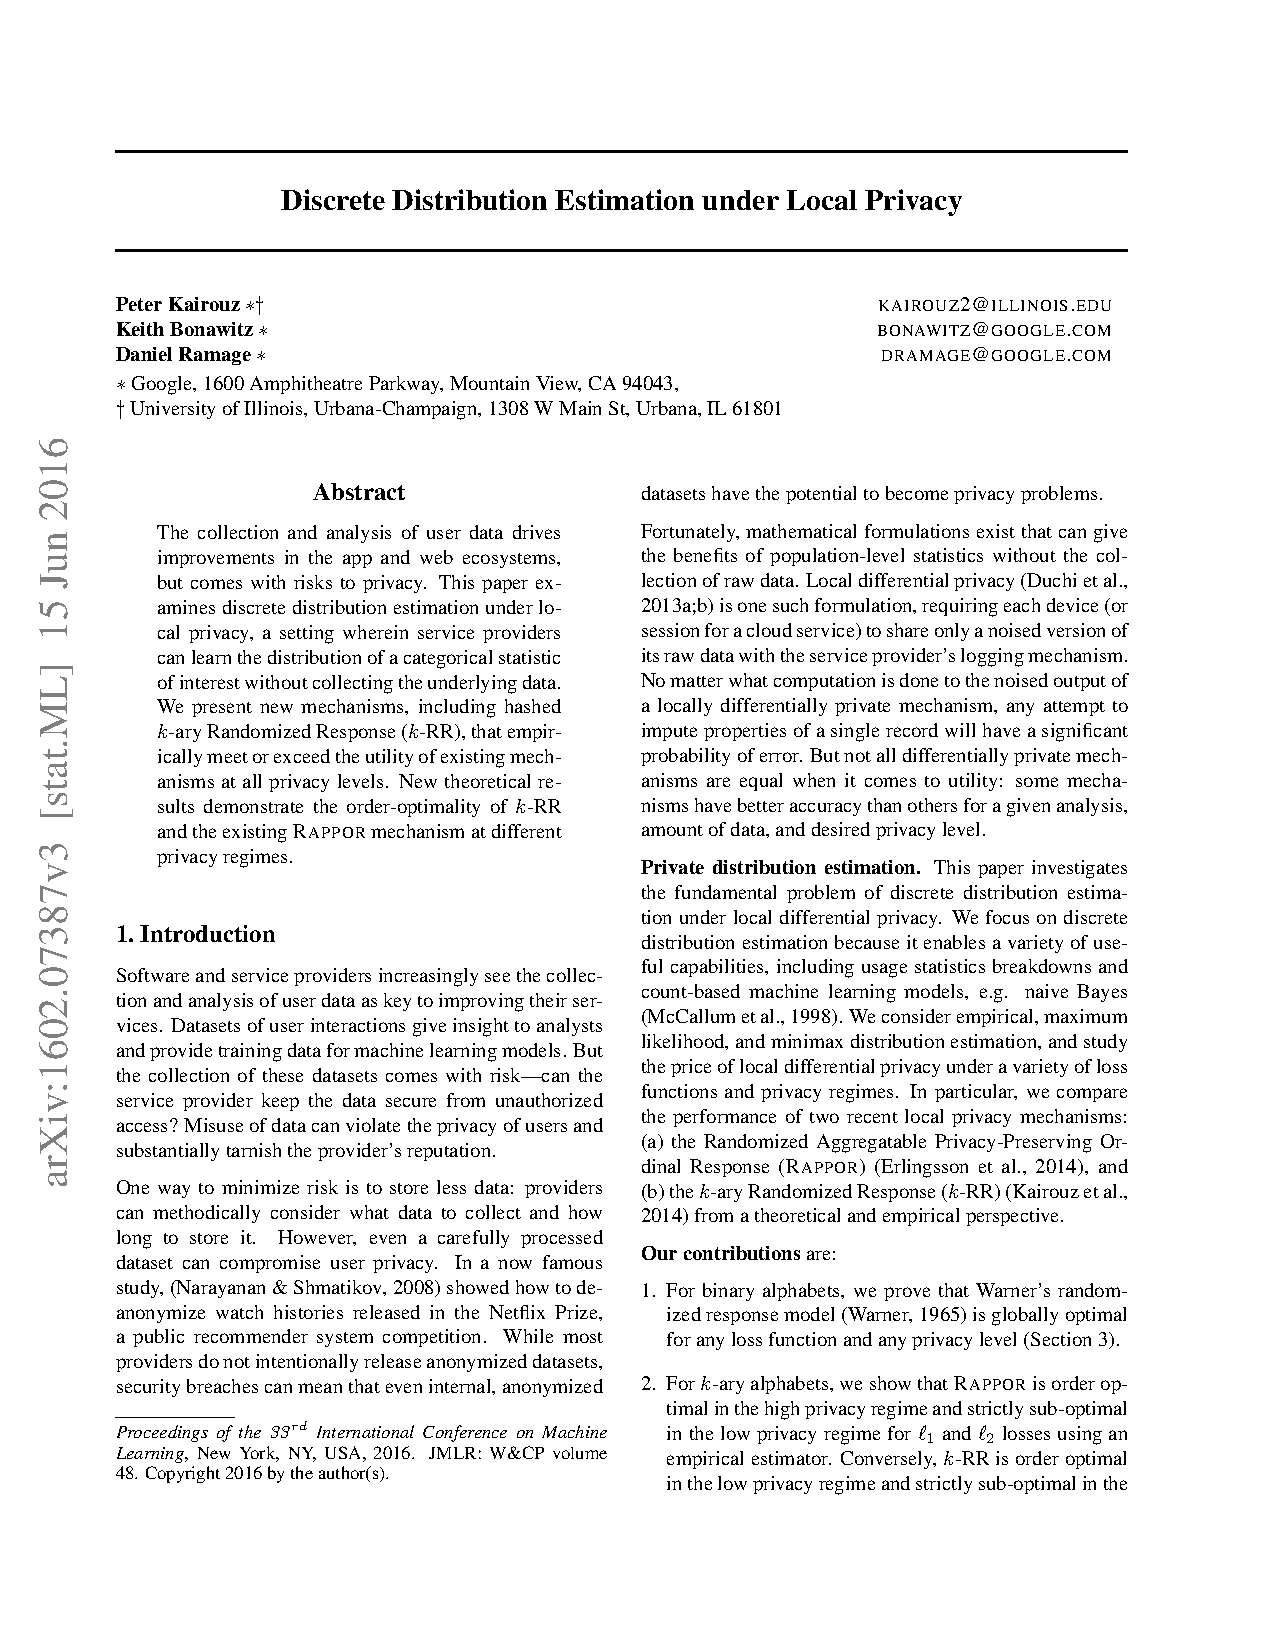
\includegraphics[width=\textwidth]{graphs/kRR.png}
    \caption{Impact of different parameters on the overall gains (first row) and normalized overall gains (second row) of the three attacks for kRR.}
    \label{fig:appendix-kRR}
\end{figure}

\begin{figure}[H]
    \centering
    \includegraphics[width=\textwidth]{graphs/oue.png}
    \caption{Impact of different parameters on the overall gains (first row) and normalized overall gains (second row) of the three attacks for OUE.}
    \label{fig:appendix-OUE}
\end{figure}

\begin{figure}[H]
    \centering
    \includegraphics[width=\textwidth]{graphs/olh.png}
    \caption{Impact of different parameters on the overall gains (first row) and normalized overall gains (second row) of the three attacks for OLH.}
    \label{fig:appendix-OLH}
\end{figure}

\end{document}

